\documentclass[11pt]{article}
\usepackage[utf8]{inputenc}
\usepackage{fullpage}
\usepackage{authblk}
\usepackage{url}
\usepackage{physics}
\usepackage{amsmath}
\usepackage{amssymb}
\usepackage{float}
\usepackage{tikz}
\usepackage{hyperref}
\usepackage{verbatim}
\usepackage[font=small,labelfont=bf, skip=1pt,center]{caption}
\DeclareMathOperator*{\minimize}{minimize}
\usepackage{bm}

%\title{AA203 Report Template}
\title{AA203 Project: Pesticide use optimization \\ Final Report}

\author{Stuart Johnson}
\affil{stujohn@stanford.edu}

\date{\today}

\begin{document}

\maketitle

\begin{abstract}
Optimizing spatio-temporal pesticide application during the growing season can have a significant impact on pesticide cost and the quantity of pesticides being applied and released into the environment. We apply optimal control techniques to a synthetic crop field and demonstrate potentially significant impact in reducing pesticide usage. The magnitude of the impact depends heavily on the details of the crop ecosystem.
\end{abstract}

\section{Introduction}
When managing a field of crops, one of the challenges is protecting the crop from consumption by pests - in particular, competing with insects for harvestable food. While there are organic practices for farming, these do not necessarily obviate the need for pesticides. In any case, it is of interest to optimize pesticide application in time and space, both from an economic and ecological health perspective. This project aims to quantify optimized pesticide application in several cases by applying the methods of optimal control. In particular, to quantify the impact of pesticide timing and spatial application in precision agriculture settings relative to exhaustive techniques - like aerial spraying of the entire field.

\section{Related Work}
Papers investigating complex (or otherwise) optimal controls in 2D for agricultural purposes are not abundant. However, there are numerous papers investigating controls for more complex combinations of pests and plants or even for irrigation control - in time and - at most - a single spatial dimension. Examples are given in \cite{R1} and \cite{R2}. Since various agricultural practices involve spatial patterns of ecosystem management - like crop rotation, for example \cite{R3}, it seems possible that the literature is missing some possible refinement of agricultural ecosystem control practices by not considering 2D scenarios.

\section{Problem Statement}
Let us suppose we are managing a crop in a square field. This crop is planted and grown for a number of months and then harvested essentially all at once (an example would be corn).

A common approach to modelling ecological problems is the reaction-diffusion (RD) equation. This allows us to model the spatial movement of chemical or biological actors and also model the life cycle and interaction of the same actors. For this project, we adopt a version of the RD equation which only models the pest as obeying spatial diffusion. The RD PDE for our crops is:

\begin{align}
	\dv{c(x,y,t)}{t} &= -k_{cp} p c + k_c \left( 1 - \frac{c}{K_c} \right) c \nonumber \\ 
	\dv{p(x,y,t)}{t} &= d_p \laplacian{p} - k_{pw} w p + k_{pc} c p - k_p p \\
	\dv{w(x,y,t)}{t} &= u - k_w w \nonumber
\end{align}

where, defined on the domain $\Omega$ of the crop field:

\begin{itemize}
\setlength\itemsep{-1pt}
\item $c(x,y,t)$ crop density ; \textbf{state}
\item $p(x,y,t)$ pest density ; \textbf{state}
\item $w(x,y,t)$ pesticide density ; \textbf{state}
\item $u(x,y,t)$ pesticide application rate ; \textbf{control}
\item $k_{cp} = 0.2$ rate of crop consumption by pest
\item $k_c = 0.1$ rate of crop growth
\item $K_c = 1.0$ carrying capacity (density) of field for crop
\item $d_p = 0.15$ diffusion coefficient of pests
\item $k_{pw} = 0.3$ rate of pest death by pesticide
\item $k_{pc} = 0.2$ rate of pest growth (requires crop)
\item $k_p = 0.025$ rate of pest death
\item $k_w = 0.2$ rate of pesticide decay - as a toxin \textit{and} as a disagreeable food additive \cite{R4}
\end{itemize}

subject to initial conditions:

\begin{itemize}
\setlength\itemsep{-1pt}
\item $c(x,y,0) = 0.5$ initial crop density ; \textbf{state}
\item $p(x,y,0) = 0.0$ initial pest density ; \textbf{state}
\item $w(x,y,0) = 0.0$ initial pesticide density ; \textbf{state}
\end{itemize}

and boundary conditions defined on the crop field boundary $\partial\Omega$:

\begin{itemize}
\setlength\itemsep{-1pt}
\item $p = 0$ homogeneous Dirichlet pest density at the boundary
\item or
\item $\nabla p(x,y,t) \cdot \hat{n} = b_p(x,y,t)$ inhomogeneous Neumann normal pest flux at the boundary
\end{itemize}

[Important note/Disclaimer: the parameters of this RD model are not necessarily indicative of actual parameters to be encountered in an any actual field of crops. Parameters were varied and sampled in such a way to yield interesting model behavior and investigate the numerical techniques involved.]

We model crop density limits via "logistic" growth in the term $k_c \left( 1 - \frac{c}{K_c} \right) c$. This limits the equilibrium crop density to $K_c$. This PDE exhibits a number of interesting growth/consumption patterns - like waves of pest density moving in response to crop consumption and pest diffusion.

Initial and boundary conditions are used to specify the nature of a pest attack during the growing season. For the purposes of the analysis below, we will assume a constant in time, spatially variable flux of pests into our crop field. This flux will specifically model a concentration of flux coming from the southeast (see Figure 4 in the Appendix) - representative of being close to a natural reservoir, for example, and some level of background flux elsewhere. The nature of the pest attack is a very important factor in the analysis.

Our problem is to optimize the spatio-temporal application of pesticide in order to minimize the impact of pests and pesticide on the crop at harvest time. This includes minimizing (see also the section on $P$ and $Q$ cost matrices below) the following:

\begin{itemize}
\setlength\itemsep{-1pt}
\item Active pesticide density across the field at harvest time
\item Pests present at harvest time
\item Crop yield loss at harvest time
\item Total pesticide application in the growing season
\end{itemize}

These are conflicting goals - for example, pesticide application both increases crop yield but also contaminates the harvested crop and the ecosystem in general.
The behavior of the PDE is strongly dependent on the parameters and initial and boundary conditions used to model the crop/pest ecosystem and the pest attack. As noted above, this model has not been calibrated or tuned to represent a realistic scenario.

\section{Approach}

The transcribed, constrained optimal control problem corresponding to the problem statement is:

\begin{align}
\minimize_{s,u} & \sum_{k=0}^{N-1} \left( (s_k - s_{goal})^T Q (s_k - s_{goal}) + u_k^T R u_k \right) \\
	     & \qquad \qquad  + (s_N - s_{goal})^T P (s_N - s_{goal}) \nonumber  \\
\text{subject to} \qquad s_0 &= \bar{s}_0 \nonumber \\
s_{k+1} &= f_d(s_k, u_k), \forall k \in \{ 0,1,\dots , N-1 \} \nonumber \\
u_k &\geq 0, \forall k \in \{ 0,1,\dots, N-1\} \nonumber \\	   
u_k &\leq u_{max}, \forall k \in \{ 0,1,\dots, N-1 \} \nonumber	     
\end{align}
 
where (see also the Experiments section):

\begin{itemize}
\setlength\itemsep{-1pt}
\item $t \in \{0, \dots N\}$
\item $s \in \mathbb{R}^{3n^2}$
\item $u \in \mathbb{R}^{n^2}$ for full control, or:
\item $u \in \mathbb{R}^{1}$ for aerial spraying control, or:
\item $\bar{s}_0$ is $c = C_0$, $p = 0$, $w = 0$
\item $C_0$ is the spatially constant crop density at time $0$
\item $s_{goal}$ is $c = C_N$, $p = 0$, $w = 0$
\item $C_N$ is crop density at harvest time $N$ assuming no pest damage (following the crop growth rate)
\end{itemize}

The cost matrices need to weight the deviation of $c$, $p$ and $w$ from their goal states in such a way to result in a desired trade-off between these costs at harvest time ($P$) and during the growing season ($Q$). After some numerical experimentation, we use the following weights for these diagonal matrices. The total weight for each section of the matrix is the product of the overall factor and the factor for $c$, $p$, $w$ and $u$.

\begin{center}
	\begin{tabular}{ | c | c | c | c | c | c | }
	\hline
    cost matrix & overall & $c$ & $p$ & $w$ & $u$ \\
    \hline
    P & 100 & 1 & 10 & .01 & 0 \\
    \hline
    Q & 0.1 & 1 & 10 & .01 & 0 \\
    \hline
    R & .001* & 0 & 0 & 0 & 1 \\
    \hline
    \end{tabular}
    \captionof{table}{Cost matrix weighting. *Note that R has an additional factor for aerial spraying.}
\end{center}

For aerial spraying, where $u \in \mathbb{R}^{1}$, we additionally weight $R$ by $n^2$ (where the spatial grid is $n \times n$) to make the penalty on the control across the field the same as it would be for a comparable spot spraying optimal control scenario.

After spatial discretization of the crop field into $n \times n$ equally spaced points (with a point on the boundaries), the PDE above is converted into a coupled system of ODEs. The Laplacian becomes a (quite sparse, block-diagonal-dominant) matrix $L$. For the purposes of this project, the Laplacian has been discretized for both 1) Dirichlet and 2) Neumann boundary conditions \cite{R5}. When homogenous (0), these boundary conditions correspond, respectively, to 1) no pest at the field boundaries or 2) a boundary impermeable to pests. As mentioned above, we will be simulating a time-constant, spatially varying boundary-normal flux of pests into our field via inhomogenous Neumann boundary conditions. Equation 1 becomes:

\begin{align}
\dot{\bm{c}} &= -k_{cp} \bm{p} \odot \bm{c} + k_c \left( 1 - \frac{\bm{c}}{K_c} \right) \odot \bm{c} \nonumber \\ 
\dot{\bm{p}} &= d_p L \bm{p} + \bm{b}_p - k_{pw} \bm{w} \odot \bm{p} + k_{pc} \bm{c} \odot \bm{p} - k_p \bm{p} \\
\dot{\bm{w}} &= \bm{u} - k_w \bm{w} \nonumber
\end{align}

where $\odot$ is the element-wise product of the vectors involved. For the purposes of our investigations, $L$ is the finite difference matrix for Neumann boundary conditions, and $\bm{b}_p$ is the boundary flux of pests, defined only on the boundary points of the spatial grid. Adding this term to an expression discretizing the Laplacian can be understood by considering the components related to the normal derivatives in the Neumann boundary condition Laplacian finite difference matrix \cite{R5}.

SCP (Sequential Convex Programming) with a trust region approach is applied to this optimal control problem. The linearized $f_d$ in the optimal control problem (2) is computed by fourth order Runge-Kutta integration. \texttt{JAX/CVXPY} are used to compute the optimal solution. As a practical computational matter, SCP with \texttt{JAX/CVXPY} is reasonably performant only to modest grid sizes. The state space ($[\bm{c};\bm{p};\bm{w}]$) is of dimension $3n^2$ and the control space ($\bm{u}$) is of dimension $n^2$ - for the full spatio-temporal control. Running SCP using the \texttt{ECOS} (the fastest tried) solver, $5 \times 5$ discretizations are relatively tractable and converge to results in a few minutes. $7 \times 7$ discretizations require hours to converge. Therefore we restrict our analyses to $5 \times 5$ grids and relatively short growth seasons. Increases in computation time make it quite challenging to explore and comprehend even a small part of the parameter space of the problem.

\section{(Numerical) Experiments}

We investigate the impact of a spatio-temporal approach to optimizing pesticide application as opposed to spatially constant, but time varying application. The latter would represent, for example, aerial spraying over the entire field. In both cases we assume a persistent pest hazard from adjacent land over the growing season. We compare pesticide quantities applied for two cases (Exp 1 and 2).

\begin{itemize}
	\setlength\itemsep{-1pt}
	\item Exp 0: Simulation of growing season with no control (no pesticide applied).
	\item Exp 1: Aerial spraying: spatially uniform application of pesticide (aerial spraying), with the time dependence to be found by optimal control. Compute total pesticide quantity applied.
	\item Exp 2: Spot spraying: optimal time and spatial pattern of pesticide application rate $u$ to be found via optimal control methods. Compute total pesticide quantity applied.
\end{itemize}

Early experiments to re-simulate the growing season in Exp 1 and 2 (after computing optimal controls) with a more accurate solver did not result in significant differences in any numerical results.

\subsection{Exp 0}

As a baseline behavior of the crops with the chosen pest flux boundary conditions and no pesticide, we show the onset of severe depletion of crops during the growing season (figure 1). This scenario defines a constant flux of pests, strongly peaked at the southeast corner of the crops (see figure 4 in the Appendix). We simulate this no pesticide situation for much longer than for Exp 1 and Exp 2 in order to get a sense of system behavior. In figure 1, we collapse time slices of the state and control to plots of statistics over the crop field (top row of the plot) or total values over time (bottom row of the plot). The min, median and max curves reflect spatial variability over the crop field. The carrying capacity of the field is shown by the dashed red line in the crop plots.

\begin{minipage}{\textwidth}
	\begin{center}
		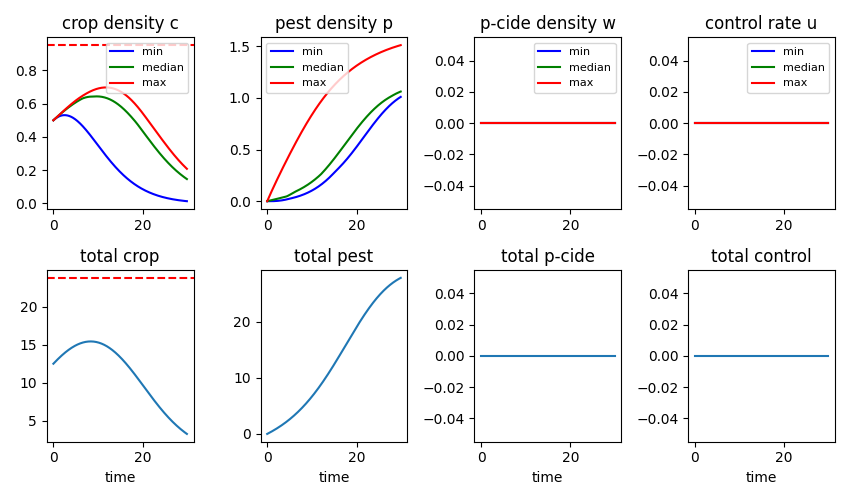
\includegraphics[width=0.8\linewidth]{../sim_240604-091905/time.png}
		\captionof{figure}{Pest attack scenario with no control. In the top row, min, median and max curves capture spatial variability. }
	\end{center}
\end{minipage}

\subsection{Exp 1: Aerial Spraying}

Aerial spraying is defined by spatially constant control - or the same spraying rate across the whole field. We find the optimal time trajectory of this control via SCP.

For Exp 1, the optimal control solution (figure 2 and  figure 5 in the Appendix) shows a mildly oscillatory control pattern, with a rise in pesticide application rate in the middle of the growing season. The optimal control problem penalizes the density of active pesticide at harvest time, so early applications of pesticide are preferred. Generally speaking, when we interchange the relative weightings of the $P$ and $Q$ cost matrices (so the terminal cost is reduced), the optimal control is non-zero much later in the growing season.

\begin{minipage}{\textwidth}
	\begin{center}
		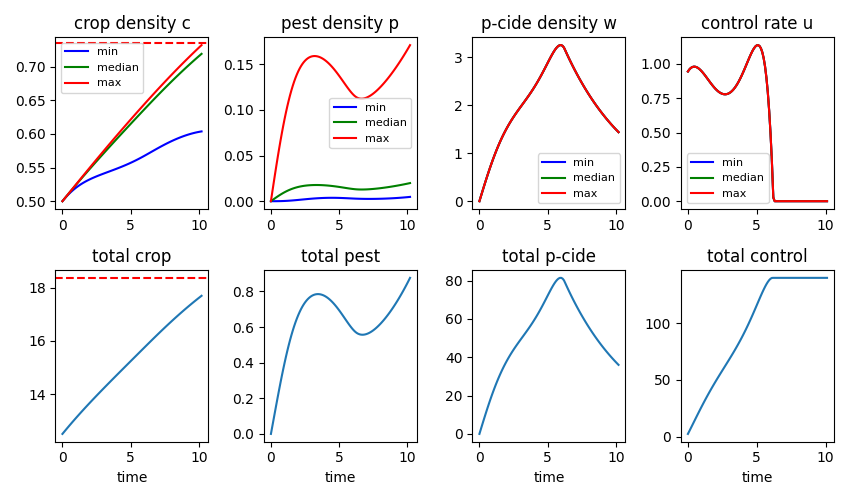
\includegraphics[width=0.8\linewidth]{../scp_240604-091225/time.png}
		\captionof{figure}{Pest attack scenario with aerial spraying control. In the top row, min, median and max curves capture spatial variability. }
	\end{center}
\end{minipage}

\subsection{Exp 2: Spot Spraying}

Spot spraying allows for complete spatial (and time) control of pesticide application.

Figure 3 and figure 6 in the Appendix show the optimal solution when spot spraying is used. While the general time trend is similar to Exp 1, the late application spike is both later in the season and concentrated in the southeast corner. The late spike in control is somewhat surprising.

In figure 3, the total control subplot is quite a bit lower than the aerial application case, and the active pesticide remaining at harvest time is less. This is reviewed in the next section.

\begin{minipage}{\textwidth}
	\begin{center}
		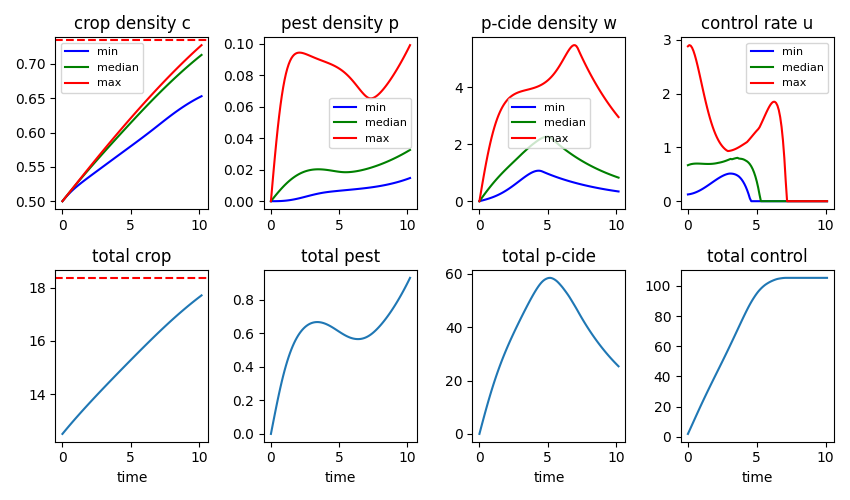
\includegraphics[width=0.8\linewidth]{../scp_240604-085334/time.png}
		\captionof{figure}{Pest attack scenario with spot spraying control. In the top row, min, median and max curves capture spatial variability. }
	\end{center}
\end{minipage}

\subsection{Aerial vs Spot application of pesticides}

Collecting the results for Exp 1 and Exp 2 at harvest time, we have:

\begin{center}
	\begin{tabular}{ | c | c | c| c| c| }
	\hline
	\multicolumn{5}{|c|}{Raw harvest-time totals} \\
	\hline
    method & crop & pest & p-cide & cumulative control \\
    \hline
    aerial & 17.70 & 0.88 & 36.02 & 139.97 \\
    \hline
    spot & 17.71 & 0.93 & 25.36 & 105.30 \\
    \hline
    \end{tabular}
\end{center}

For the same crop yield, \textit{for this combination of crop ecosystem parameters}, optimal spot application requires $(139.97-105.30)/139.97 = 25\%$ less pesticide than spatially constant aerial spraying over the entire field. Harvest quality, in terms of active pesticide on the crops, is also significantly better in spot spraying. This result depends heavily on numerous ecosystem parameters, such as the pest diffusion rate $d_p$. Pests with more mobility rapidly decrease the spot spraying advantage. It is also possible our selection of quadratic losses is favoring aerial spraying (see the conclusions section).

\section{Conclusions and Future Work}

Optimal control is capable of computing optimal spatio-temporal pesticide application strategies which could achieve large savings in pesticides for the same crop yield and quality of harvested crop. Solving the optimal control problem in 2D and time is a challenge for the implementation of Sequential Convex Programming applied here. It would be interesting to understand the limits of SCP for this PDE, and explore other solution techniques.

The optimal controls obtained via SCP appear to have some unexpected control patterns in time - utlizing pulses of control activity. Are there also some subtle control patterns occurring spatially? Further investigation of the parameter space is warranted to investigate this. In order to apply these controls to actual crop management, we would also need to integrate the detection of pest infestations into our control strategy - unless pest attack patterns were quite repeatable!

We also have not investigated various control constraints, like limits on pesticide application rate and timings. Presumably aerial control is not done continuously!

Comparing results for two different optimal control scenarios can be problematic. In our case, we are using the same cost function for two control scenarios which can have different optimal spatio-temporal behavior. One wonders, for example, if the quadratic cost disfavors the spot spraying approach, which can take advantage of large local departures from the target behavior; the quadratic cost function will selectively penalize larger departures. This argues for a Linear Programming approach, but attempts at this with \texttt{JAX/CVXPY} indicated \textit{much} slower convergence.

Even though this method can reduce pesticide usage for some pest attack scenarios, more ecologically sound practices would rely on more subtle and natural methods of pest control. It would be interesting to investigate these techniques (e.g., EBPM \cite{R3}) in terms of optimal control. These methods can rely on the spatial relationships between parts of the managed ecosystem, and so may argue for optimization via spatio-temporal optimal control. At a minimum, more complex dynamics models would be needed; EBPM depends on establishing a more complex ecosystem to maintain the harvest compromise. 

% ----------

%\bibliography{refs}
%\bibliographystyle{plain}

\begin{thebibliography}{1}
\bibitem{R1} Ihza Rizkia Fitri, Faruda Hanum, Ali Kusnanto, Toni Bakhtiar, \textbf{Optimal Pest Control Strategies with Cost-effectiveness Analysis}, \textit{The Scientific World Journal, Hindawi Publishing Corporation}, 21 April 2021.
\bibitem{R2} Fernando Lobo Pereira, Fernando Arménio Fontes, Maria Margarida Ferreira, 
Maria do Rosário Pinho, Vilma Alves Oliveira, Eduardo Costa, and Geraldo Nunes Silva, \textbf{Conference Paper: An Optimal Control Framework for Resources Management in Agriculture}, \textit{Hindawi Publishing Corporation, Conference Papers in Mathematics},  14 July 2013.
\bibitem{R3} Miguel A. Altieri, Clara I. Nichols, and Marlene A. Fritz, 
\textbf{Manage Insects on Your Farm: A Guide to Ecological Strategies},
\textit{Sustainable Agriculture Research and Education (SARE)}, 2005.
\bibitem{R4} National Pesticide Information Center, \textbf{http://npic.orst.edu/factsheets/half-life.html}
\bibitem{R5} Stefan Bilbao,
\textbf{Numerical Sound Synthesis: Finite Difference Schemes and Simulation in Musical Acoustics, Chapter 10},
\textit{Wiley}, 2009.
\end{thebibliography}


\section{Appendix}

Plots of spatial patterns for each of the experiments are here to save space at the beginning of the document.

\subsection{Exp 0: No control}

\begin{minipage}{\textwidth}
	\begin{center}
		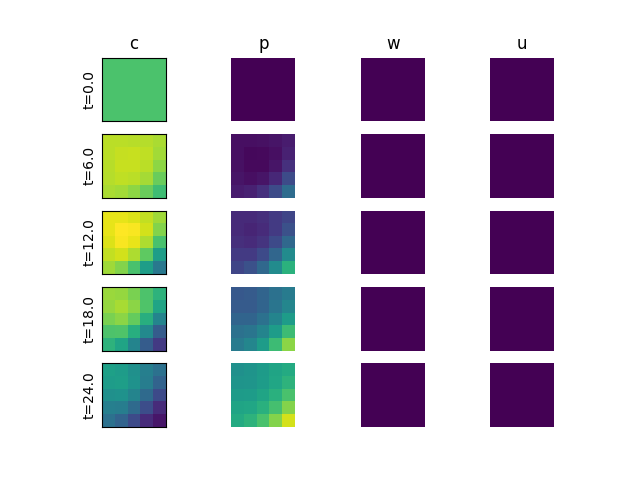
\includegraphics[width=0.8\linewidth]{../sim_240604-091905/slices.png}
		\captionof{figure}{Pest attack scenario with no control. c= crop density, p = pest density, w = pesticide density, u = pesticide application rate}
		\vspace{5pt}
	\end{center}
\end{minipage}


\subsection{Exp 1: Aerial Spraying}

\begin{minipage}{\textwidth}
	\begin{center}
		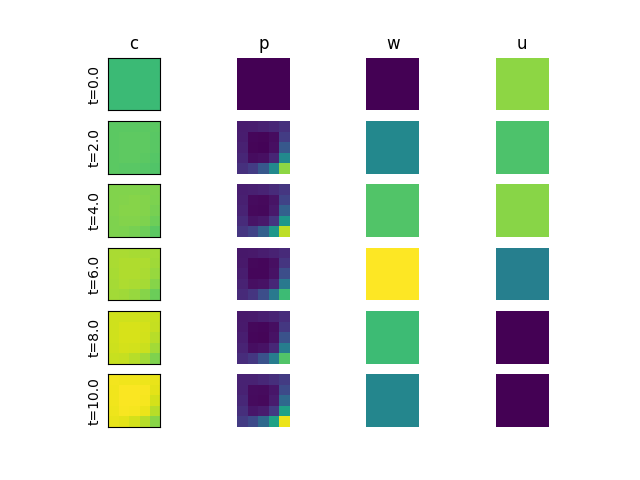
\includegraphics[width=0.8\linewidth]{../scp_240604-091225/slices.png}
		\captionof{figure}{Pest attack scenario with aerial spraying control: spatial slices.  c= crop density, p = pest density, w = pesticide density, u = pesticide application rate}
		\vspace{5pt}
	\end{center}
\end{minipage}


\subsection{Exp 2: Spot Spraying}

\begin{minipage}{\textwidth}
	\begin{center}
		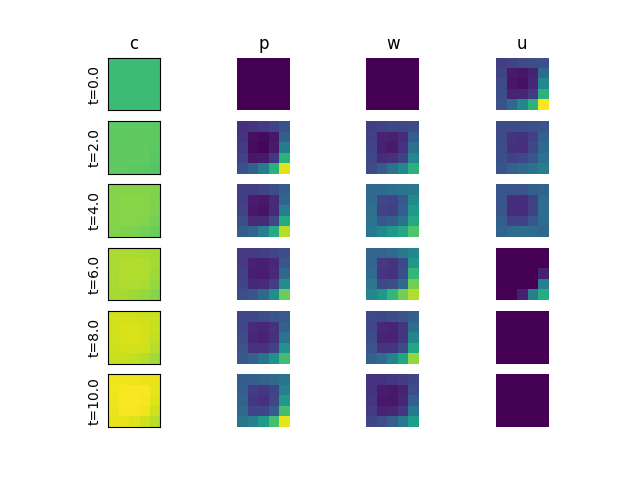
\includegraphics[width=0.8\linewidth]{../scp_240604-085334/slices.png}
		\captionof{figure}{Pest attack scenario with spot spraying control: spatial slices. c= crop density, p = pest density, w = pesticide density, u = pesticide application rate}
		\vspace{5pt}
	\end{center}
\end{minipage}


\section{Code}

See the public github repo: \href{https://github.com/StuartGJohnson/AA203\_project}{https://github.com/StuartGJohnson/AA203\_project}.

\end{document}
